

\begin{figure*}[ht!]
	\centering
	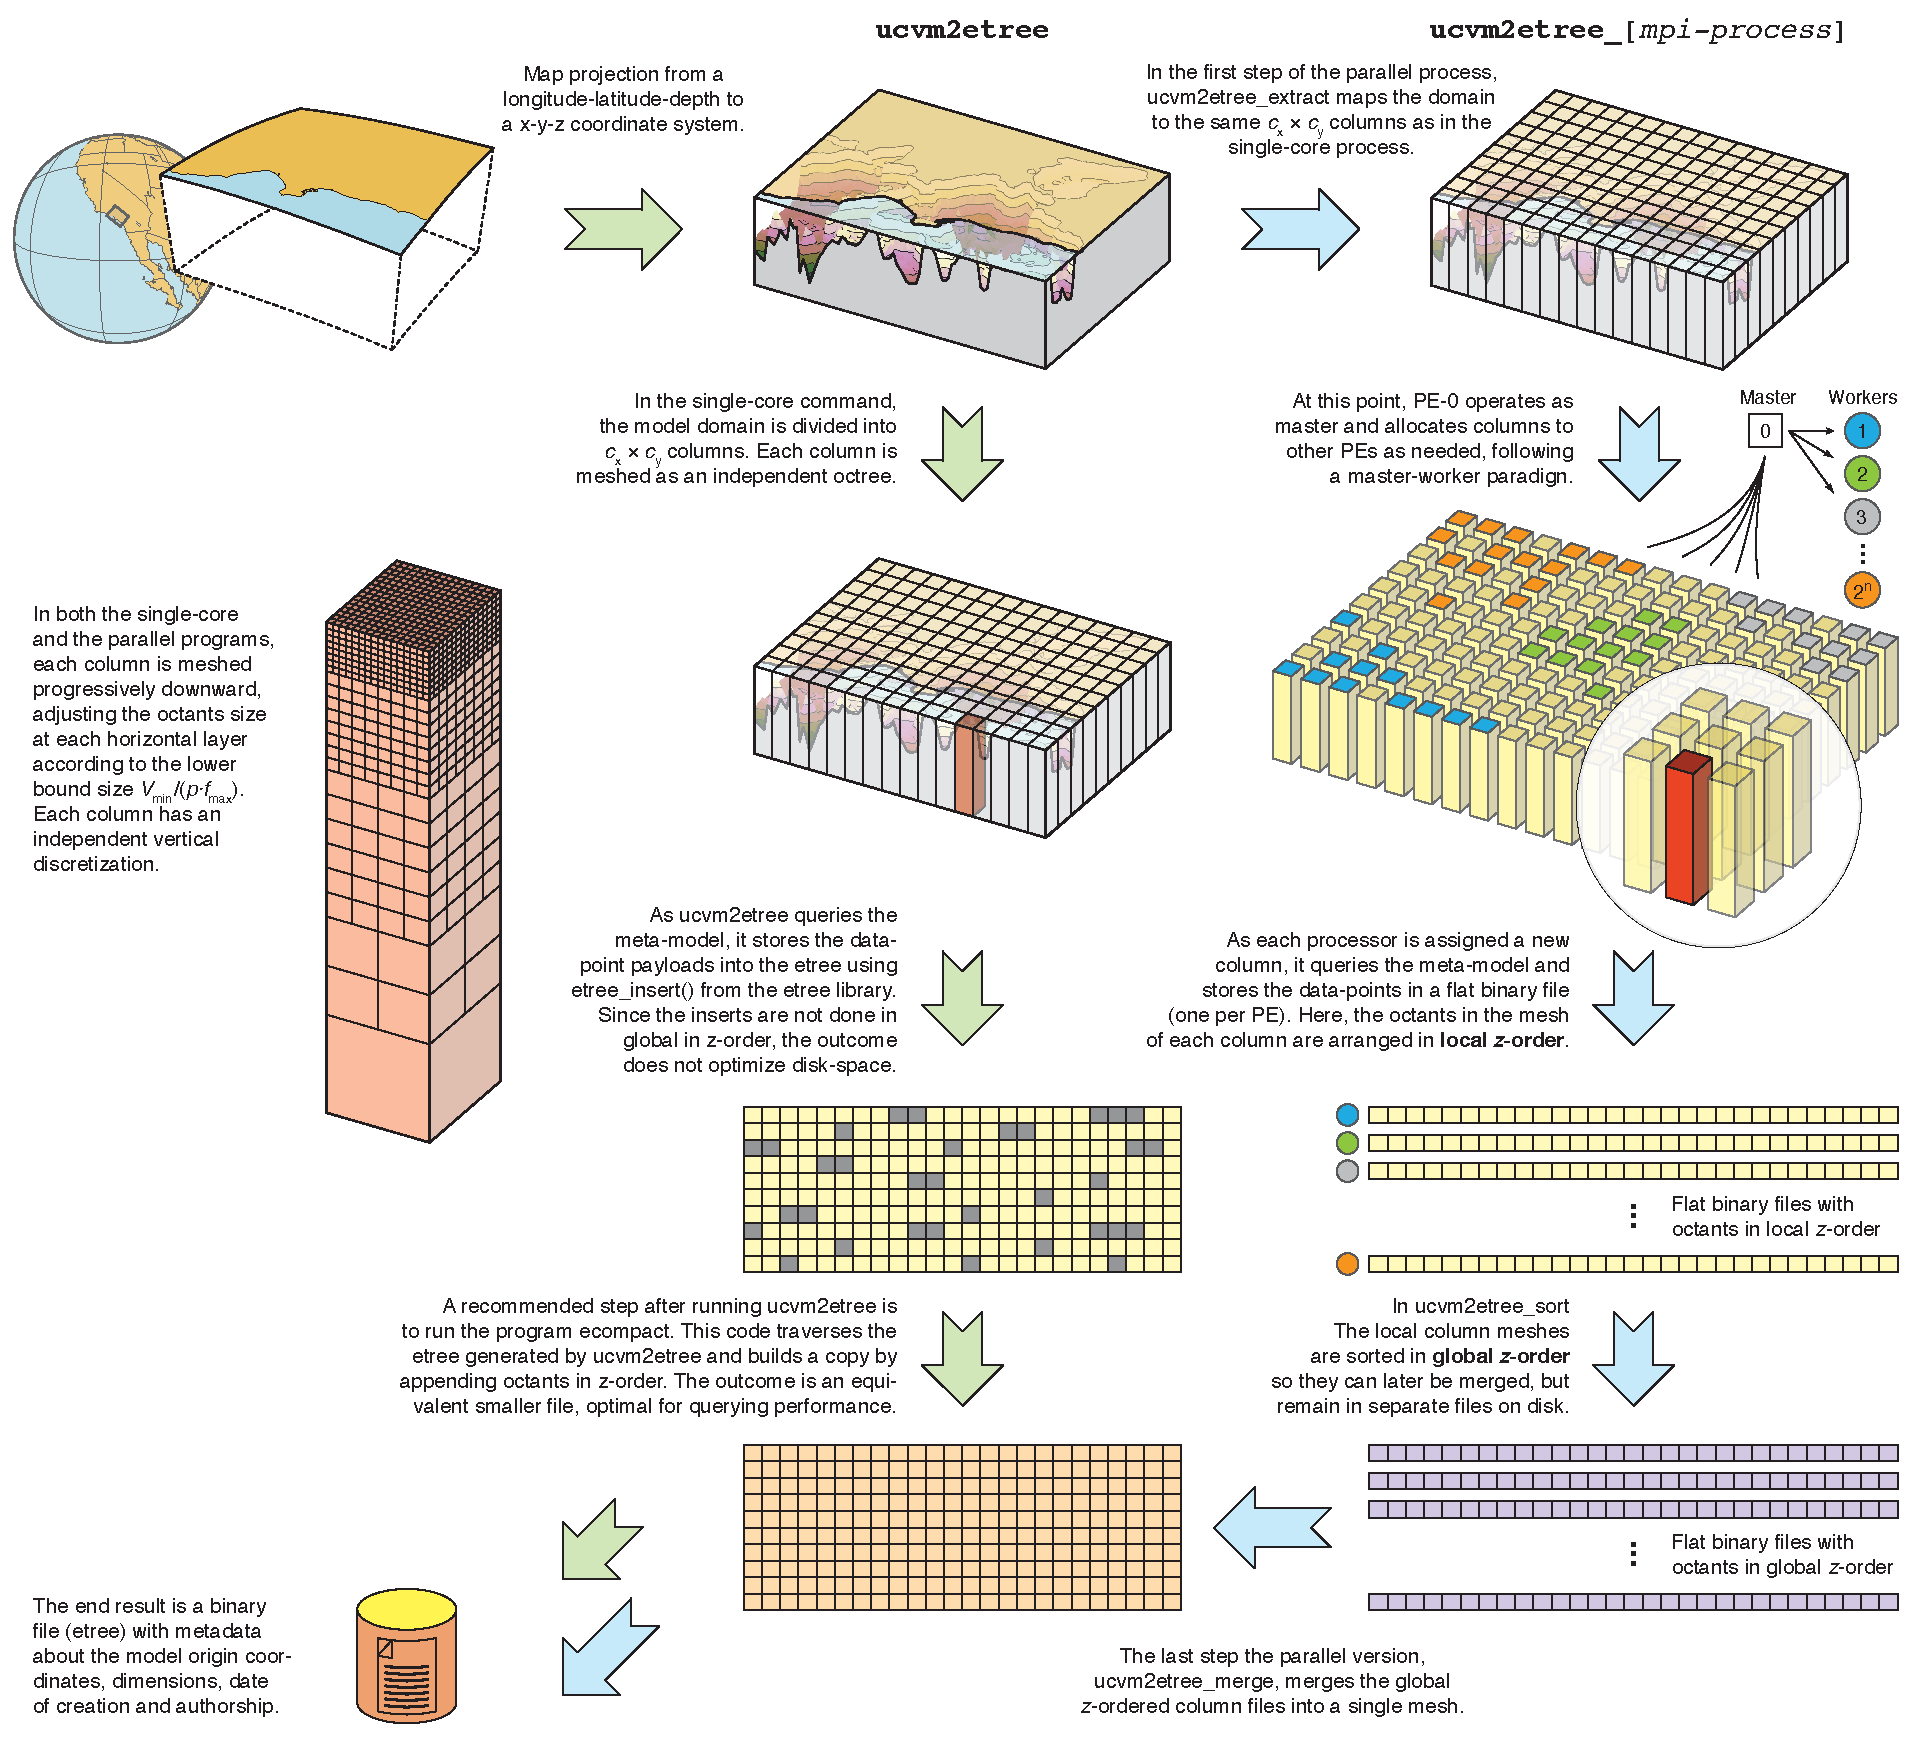
\includegraphics
		[width=\textwidth]
		{figures/pdf/ucvm-to-etree}
	\caption{Construction of an semi-unstructured mesh in the Etree database format using the program \texttt{ucvm2etree} (green arrows); and its MPI equivalent process controlled by the programs \texttt{ucvm2etree\_extract}, \texttt{ucvm2etree\_sort} and \texttt{ucvm2etree\_merge} (blue arrows). Note that in contrast to the structured grid construction process, here the information payload (\vs{}, \vp{}, and $\rho$) is associated with the octants in the octree structure and not with a point. In other words, the querying and assignment process mapps the information queried at the center of each octant to the whole volume enclosed by the octant.}
	\label{fig:etrees}
\end{figure*}
% ---------------------------------------------------------------------------------------------


\subsection{Hercules}

The framework may also be utilized to generate a semi-unstructured octree in the \textit{etree} database format \citep{Tu_2003_Tech} suitable for use with the Hercules earthquake simulation software, using the command-line program \texttt{ucvm2etree}.

The construction of an etree proceeds as shown in Figure \ref{fig:etrees}, which follows some of the basic ideas first proposed in the implementation by \citet{Taborda_2007_Proc}. The user specifies the extents of the etree by describing the $x$-$y$-$z$ dimensions of the domain in meters, as well as providing the geographical data necessary to define a bounding box on the Earth's surface. In the case of the Hercules format, this consists of the geographic coordinates of the four corners of the bounding box. In the case of the SCEC format, this is done similarly as in the case of the structured meshes explained before. Using the corresponding bilinear or Proj.4 projection, this surface bounding box is mapped to the $x$-$y$ plane of the domain. The $z$ dimension of the domain is interpreted as depth from the free surface. In this way, any ($x,y,z$) coordinate in the domain may be transformed to a (\textit{latitude},\,\textit{longitude},\,\textit{depth}) coordinate relative to the Earth's surface. It is assumed that the user has pre-computed the domain dimensions such that they reflect the actual distances in the geographic bounding box (using any preferred projection or spheroid model). Note, however, that the octree format places restrictions on the possible valid domain sizes \citep{Tu_2003_Tech, Taborda_2007_Proc}.

This domain is then spatially decomposed at a coarse-grained level, dividing the volume into a two-dimensional logical grid of rectangular cuboids (columns) aligned with the $x$-$y$ plane of the original domain, with each column having a fixed size. With this coarse decomposition complete, each column of the original domain may then be processed in sequence by \texttt{ucvm2etree}, or in parallel, as is the case with the MPI version of this utility (see Figure \ref{fig:etrees}).

This fine-grain decomposition into octants is an adaptive process that depends on the shear-wave velocities (\vs{}) encountered within that column as well as four parameters provided by the user: \vsmin{}, a floor \vs{} for purposes of bounding octant sizes to a minimum size; \fmax{}, the maximum simulation frequency to support; $p$, the desired number of points per wavelength to be used in a simulation model; and $s_{_{\max}}$, the maximum octant size to allow. Based on these parameters, the program determines the range of octant sizes to allow within a column. The upper bound is determined by:
%
\begin{equation}
\label{eq:octant_upper}
	s_{_{\mathrm{upper}}} = \min \left( l_c, s_{_{\max}} \right)
	\hspace{0.3em},
\end{equation}
%
where $l_c$ is the column length. The lower bound is given by:
%
\begin{equation}
\label{eq:octant_lower}
	s_{_{\mathrm{lower}}} = \frac{ V_{\mathrm{S}_{\min}} }{ p f_{_{\max}}}
	\hspace{0.3em}.
\end{equation}
%
As the octree format places constraints on valid octant sizes, these two bounds are normalized with the relation:
%
\begin{equation}
\label{eq:octant_size}
	s_{_{\mathrm{octant}}} = \frac{ l_d }{ 2^{ \left( \left\lceil \log_{2} \left( \frac{l_d}{s} \right) \right\rceil \right)} }
	\hspace{0.3em}.
\end{equation}
%
Here, the variable $l_d$ is the domain length (longest side); and the variable $s$ is the size to normalize, which is either $s_{_{\mathrm{upper}}}$ or $s_{_{\mathrm{lower}}}$, corresponding to the upper and lower bounds, respectively.

With these bounds established, the program successively queries two-dimensional slices of octants, starting at the column surface and stepping downward to greater depths. Initially, the octants are of size $s_{_{\mathrm{lower}}}$ (maximum resolution). Then, as the program progresses downwards, the octants are resized based on the actual \vs{} values encountered within a slice. After each slice is queried, the minimum \vs{} found within is inserted into equation (\ref{eq:octant_lower}) and then normalized with (\ref{eq:octant_size}) to yield an updated octant size. If this new size differs from the current size while still falling within the $s_{_{\mathrm{lower}}}$ and $s_{_{\mathrm{upper}}}$ bounds, and if this size fits in the remaining vacant space of the octree, then the slice is re-queried at the new size. Otherwise, the slice of octants is accepted as queried and inserted into the etree database.

The MPI implementation of \texttt{ucvm2etree} is a workflow consisting of three programs: \texttt{ucvm2e\-tree\_extract}, \texttt{ucvm2etree\_sort}, and \texttt{ucvm2etree\_merge}. The program \texttt{ucvm2etree\_extract} performs the same spatial decomposition and velocity model querying as described above, with the change that it employs a master-worker paradigm to parallelize column extraction. As the shear wave velocity can vary dramatically across columns, the number of octants in each column may also vary considerably. This paradigm allows for a limited form of load balancing among processing elements in the job. The master processing element, rank 0, consecutively assigns columns to idle workers, with the worker pool being the remaining processing elements within the job. Each worker, in turn, extracts its assigned column(s) from the meta-model independently of the other workers, and the octants are temporarily saved to disk in a flat binary file, one file per worker process. Columns are assigned in this manner until all have been successfully extracted and saved. The program \texttt{ucvm2etree\_sort} locally sorts the octants within each octant file by their location code. The last program in the workflow, \texttt{ucvm2etree\_merge}, performs a merge of the locally sorted octant files, such that rank 0 inserts the ordered octants one at a time into the etree database \citep[in its natural $z$-order; see][]{Tu_2003_Tech}. Since the octants are globally sorted at this point, the insertion is simply an append operation. 


